%
% 1-lagrangemult.tex
%
% (c) 2023 Prof Dr Andreas Müller
%
\section{Lagrange-Multiplikatoren für Variationsprobleme
\label{buch:nebenbedingungen:section:lagrangemult}}
\kopfrechts{Lagrange-Multiplikatoren für Variationsprobleme}
In diesem Abschnitt gehen wir wieder von einem Funktional
\begin{equation}
I(y)
=
\int_{x_1}^{x_2}
F(x,y(x),y'(x))
\,dx,
\label{buch:nebenbedingungen:lagrangemult:eqn:}
\end{equation}
für das eine Funktion $y(x)$ mit Randbedingungen $y(x_1)=y_1$ und
$y(x_2)=y_2$ gesucht wird, deren Wert $I(y)$ extremal ist.
Für dieses Problem wurde als notwendige Bedingung für die Lösung die
Euler-Lagrange-Differentialgleichung gefunden.
In diesem Abschnitt sollen jetzt zusätzliche Bedingungen auferlegt 
werden, zum Beispiel vorgegebene Werte in vorgegebenen Punkten oder
vorgegebene Werte eines Funktionals.
In
Abschnitt~\ref{buch:nebenbedingungen:lagrangemult:subsection:nebenbedingungen}
soll gezeigt werden, wie sich sollche Nebenbedingungen formulieren
lassen.
Die Euler-Lagrange-Differentialgleichung entstand aus der Idee
der Richtungsableitung, die auch bei der Herleitung der Methode
der Lagrange-Multiplikatoren im Mittelpunkt stand.
Im
Abschnitt~\ref{buch:nebenbedingungen:lagrangemult:subsection:einzeln}
wird das Problem für eine einzelne Nebenbedingung gelöst, in
Abschnitt~\ref{buch:nebenbedingungen:lagrangemult:subsection:lagrangemult}
dann für eine endliche Anzahl von Nebenbedingungen, wobei ein der
Methode der Lagrange-Multiplikatoren ähnliches Lösungsverfahren entsteht.

%
% Nebenbedingungen für Variationsprobleme
%
\subsection{Nebenbedingungen für Variationsprobleme
\label{buch:nebenbedingungen:lagrangemult:subsection:nebenbedingungen}}
In diesem Abschnitt zeigen wir, dass sich verschiedene naheliegende
Nebenbedingungen an Funktionen in einem Variationsproblem allgemein
als Nebenbedingungsfunktionale der gleichen Art wie das zu minimierende
Funktional formulieren lassen.

%
% Integrale als Nebenbedingungen
%
\subsubsection{Integrale als Nebenbedingungen}
Der Sage nach soll Dido, Tochter des tyrischen Königs Mattan, auf der
Flucht vor ihrem Bruder Pygmalion über Zypern am Golf von Tunis 
gelandet sein.
\index{Dido}%
\index{Mattan}%
\index{Pygmalion}%
\index{Tunis}%
Der Numiderkönig Iarbas soll ihr so viel Land versprochen haben, wie
sie mit einer Kuhhaut umspannen konnte.
\index{Iarbas}%
Dido schnitt die Haut in einen dünnen Streifen und konnte damit ein
Gebiet umspannen, das das Gebiet der Byrsa, der Burg des späteren
Karthago umfasste.
\index{Byrsa}%
\index{Karthago}%

Dieser Mythos impliziert, dass Karthago als Lösung eines sogenannten
isoperimetrischen Problems gegründet wurde.
\index{isoperimetrisch}%
Im konkreten Fall geht es zum Beispiel darum, eine Funktion $y(x)$
auf dem Intervall $[x_1,x_2]$ zu finden, welche $y(x_1)=y(x_2)=0$,
die den Flächeninhalt
\[
I(y)
=
\int_{x_1}^{x_2} y(x)\,dx
\]
maximiert.
Die Länge der Kurve ist
\[
l(y)
=
\int_{x_1}^{x_2}
\sqrt{1+y'(x)^2}
\,dx
=
L
\]
dabei vorgeben.

%
% Vorgegebene Werte
%
\subsubsection{Vorgegebene Werte}
Wir betrachten zunächst den Fall einer Bedingung, dass an einer Stelle
$x_*$ der Werte $y_*=y(x_*)$ der Lösungsfunktion $y(x)$ vorgegeben ist.
Auch diese Art von Nebenbedingung kann als Integral geschrieben werden.
Dazu wird die Ableitung $y'(x)$ integriert und erhält
\[
J(y)
=
\int_{x_1}^{x_*} y'(x)\,dx
=
\biggl[y(x)\biggr]_{x_1}^{x_*}
=
y(x_*)-y(x_1).
\]
Das Integral kann mit der Heaviside-Funktion
\begin{equation}
\vartheta(x)
=
\begin{cases}
1&\qquad x\ge 0\\
0&\qquad\text{sonst}
\end{cases}
\label{buch:nebenbedingungen:lagrangemult:eqn:heaviside}
\end{equation}
geschrieben werden.
Die Funktion $x\mapsto\vartheta(x_*-x)$ verschwindet genau dann,
wenn $x_*\ge x$ ist.
Daher ist
\[
J(y)
=
\int_{x_1}^{x_*} y'(x)\,dx
=
\int_{x_1}^{x_2} y'(x)\vartheta(x_*-x)\,dx.
\]
Mit der Lagrange-Funktion
\begin{equation}
G(x,y,y')
=
\vartheta(x_*-x)
y'
\label{buch:nebenbedingungen:lagrangemult:eqn:heavilagrange}
\end{equation}
wird $J(y)$ zu einem Funktional
\[
J(y)
=
\int_{x_1}^{x_2}
G(x,y(x),y'(x))
\,dx.
\]
Die einzige Schwierigkeit ist, dass die Funktion $G(x,y,y')$ nicht
differenzierbar ist in der ersten Variablen.

Die Forderung, dass $J(y)$ einen vorgegebenen Wert $g$ annehmen muss,
kann weiter vereinfacht werden.
Ersetzt man die Funktion $G$ durch $\tilde{G}(x,y,y')=G(x,y,y')-g/(x_1-x_1)$,
dann wird das Funktional
\begin{align*}
\tilde{J}(y)
&=
\int_{x_1}^{x_2}
\tilde{G}(x,y(x),y'(x))\,dx
\\
&=
\int_{x_1}^{x_2} G(x,y(x),y'(x)) - \frac{g}{x_2-x_1}\,dx
\\
&=
J(y) - g
=
0.
\end{align*}
Es genügt also, Nebenbedingungen der Form
\[
\int_{x_1}^{x_2} G(x,y(x),y'(x))\,dx = 0
\]
zu betrachten.

%
% Ableitung der Heaviside-Funktion
%
\subsubsection{Ableitung der Heaviside-Funktion}
Mit der Theorie der Distributionen lässt sich die Schwierigkeit,
dass $G(x,y,y')$ nicht differenzierbar ist, umgehen.
Da es bei der Herleitung der Euler-Lagrange-Differentialgleichung nur
auf Integrale von Produkten mit beliebig oft stetig differenzierbaren
Funktionen ankommt, lässt sich die Ableitung der Heaviside-Funktion
als Dirac-\textdelta-Funktion
\[
\vartheta'(x-x_*) = \delta(x-x_*)
\]
an der Stelle $x_*$ schreiben.
Das Integral eines Produktes einer Funktion $f(x)$ mit der
Delta-Funktion an der Stelle $x_*$ liefert
\[
\int_{x_1}^{x_2} \delta(x-x_*) f(x)\,dx
=
f(x_*),
\]
den Wert des Faktors $f(x)$ an dieser Stelle.
Damit bleibt die Formel für die partielle Integration erhalten,
wie wir im folgenden nachrechnen wollen.
Dazu berechnen wir das Integral des Produktes $\vartheta(x-x_*)f'(x)$
direkt als
\begin{align}
\int_{x_1}^{x_2}
\vartheta(x_*-x) f'(x)
\,dx
&=
f(x_*)-f(x_1)
\label{buch:nebenbedingungen:lagrangemult:eqn:lhs}
\intertext{und andererseits die beiden Terme auf der rechten Seite der
Regel für das partielle Integrieren, die}
\biggl[\vartheta(x_*-x) f(x)\biggr]_{x_1}^{x_2}
&=
\underbrace{\vartheta(x_*-x_2)}_{\displaystyle = 0}
f(x_2)
-
\underbrace{\vartheta(x_*-x_1)}_{\displaystyle = 1}
f(x_1)
=
-f(x_1)
\notag
\\
\int_{x_1}^{x_2}
\delta(x-x_*)f(x)\,dx
&=
f(x_*)
\notag
\intertext{sind.
Die rechte Seite von~\ref{buch:nebenbedingungen:lagrangemult:eqn:lhs}
ist daher dasselbe wie
}
\int_{x_1}^{x_2}
\vartheta(x_*-x) f'(x)
\,dx
&=
\biggl[\vartheta(x_*-x) f(x)\biggr]_{x_1}^{x_2}
-
\int_{x_1}^{x_2}
\vartheta'(x-x_*)f(x)\,dx.
\end{align}
Dies zeigt, dass die Regel für das partielle Integrieren auch
für die Funktion $\vartheta$ gilt, sofern sie nur
als Faktor zusammen mit differenzierbare Funktionen verwendet wird.
Da genau diese Situation in der Herleitung der
Euler-Lagrange-Differentialgleichung vorliegt, lässt sich diese auf
Funktionale mit einer Lagrange-Funktion wie 
\eqref{buch:nebenbedingungen:lagrangemult:eqn:heavilagrange}
verallgemeinern.

%
% Allgemeine Form von Nebenbedingungen
%
\subsubsection{Nebenbedingungsfunktionale}
Die beiden Beispiele illustrieren, dass sich Nebenbedingungen für
Variationsprobleme meistens in der Form eines Nebenbedingungsfunktionls
schreiben kann.
Eine Nebenbedingung ist also gegeben durch eine Lagrange-Funktion
\[
G
\colon
\mathbb{R}
\times
\mathbb{R}
\times
\mathbb{R}
\to
\mathbb{R}
:
(x,y,y')
\mapsto
G(x,y,y')
\]
und den Wert, $g$, den das Funktional
\[
\int_{x_1}^{x_2}
G(x,y(x),y'(x))\,dx
=
g
\]
annehmen muss.

%
% Eine einzelne Nebenbedingung
%
\subsection{Eine einzelne Nebenbedingung
\label{buch:nebenbedingungen:lagrangemult:subsection:einzeln}}
Wie im Abschnitt~\ref{buch:fuvar:section:nebenbedingungen} betrachten
wir zunächst den etwas übersichtlicheren Fall einer einzelnen Nebenbedingung.

\begin{aufgabe}
\label{buch:nebenbedingungen:lagrangemult:aufgabe:eine}
Man finde eine Funktion $y\colon[x_1,x_2]\to\mathbb{R}$ mit $y(x_1)=y_1$
und $y(x_2)=y_2$, die das Funktional
\[
I(y)
=
\int_{x_1}^{x_2} F(x,y(x),y'(x))\,dx
\]
unter der Nebenbedingung
\[
\int_{x_1}^{x_2} G(x,y(x),y'(x))\,dx = 0
\]
extremal macht.
\end{aufgabe}

Über die Funktionen $F$ und $G$ nehmen wir an, dass sie alle stetigen
Differenzierbarkeitseigenschaften haben, die für die nachfolgenden
Rechnungen benötig werden.

Die Herleitung der Euler-Lagrange-Differentialgleichung für das
Funktional $I(y)$ verwendet eine beliebig oft differenzierbare 
Funktion $\eta(x)$ mit $\eta(x_1)=\eta(x_2)=0$ und bildet
die Richtungsableitung
\[
\frac{d}{d\varepsilon}
I(y+\varepsilon \eta)
\bigg|_{\varepsilon=0}
=
\frac{d}{d\varepsilon}
\int_{x_1}^{x_2}
F(x,y(x)+\varepsilon\eta(x),y'(x)+\varepsilon \eta'(x))\,dx
\bigg|_{\varepsilon=0}
\]
ausgehend von einer angenommenen Lösung $y(x)$.
Für die Aufgabe~\ref{buch:nebenbedingungen:lagrangemult:aufgabe:eine}
reicht dies jedoch nicht, denn es ist nicht garantiert, dass die
Funktionen $y+\varepsilon\eta$ die Nebenbedingung erfüllen.
Es ist also eine kompliziertere Parametrisierung $y(x,\varepsilon)$
der Nachbarfunktionen nötig, mit denen die Ableitung
\begin{align*}
\frac{d}{d\varepsilon}I(y(x,\varepsilon))
&=
\frac{d}{d\varepsilon}
\int_{x_1}^{x_2}
F(x,y(x,\varepsilon),y'(x,\varepsilon))\,dx
\end{align*}
gebildet werden kann.
Dabei soll $y'(x,\varepsilon)$ die partielle Ableitung nach $x$ 
bezeichnen, es soll $y(x,0)=y(x)$ sein und es soll $y(x_1,\varepsilon)=y_1$
und $y(x_2,\varepsilon)=y_2$
für alle in Frage kommenden Werte von $\varepsilon$ gelten.
Weiter müssen die Funktionen $x\mapsto y(x,\varepsilon)$ die Nebenbedingung
\[
J(y(x,\varepsilon))
=
\int_{x_1}^{x_2} G(x,y(x,\varepsilon),y'(x,\varepsilon))\,dx
=
0
\]
für alle $\varepsilon$ erfüllen.

Jetzt muss die Ableitung der Funktionale $I$ und $J$ nach $\varepsilon$
an der Stelle $\varepsilon =0$ berechnet werden.
Die Rechnung ist für beide Funktionale gleich, im folgenden wird sie
nur für $J$ ausgeschrieben.
Die Ableitung nach $\varepsilon$ ist
\begin{align*}
\frac{d}{d\varepsilon}
J(y(x,\varepsilon))
&=
\frac{d}{d\varepsilon}
\int_{x_1}^{x_2}
G(x,y(x,\varepsilon),y'(x,\varepsilon))\,dx
\\
&=
\int_{x_1}^{x_2}
\frac{\partial G}{\partial y}(x,y(x,\varepsilon),y'(x,\varepsilon))
\frac{\partial y}{\partial\varepsilon}(x,\varepsilon)
+
\frac{\partial G}{\partial y'}(x,y(x,\varepsilon),y'(x,\varepsilon))
\frac{\partial y'}{\partial\varepsilon}(x,\varepsilon)
\,dx.
\intertext{An der Stelle $\varepsilon=0$ schreiben wir für $\eta(x)$ für
die partielle Ableitung von $y(x,\varepsilon)$ nach $\varepsilon$ und
erhalten}
\frac{d}{d\varepsilon}
J(y(x,\varepsilon))
\bigg|_{\varepsilon=0}
&=
\int_{x_1}^{x_2}
\frac{\partial G}{\partial y}(x,y(x),y'(x))
\eta(x)
+
\frac{\partial G}{\partial y'}(x,y(x),y'(x))
\eta'(x)
\,dx.
\intertext{Da $\eta(x_1)=\eta(x_2)=0$ ist, kann der zweite Term mit
partieller Integration in}
&=
\int_{x_1}^{x_2}
\biggl(
\frac{\partial G}{\partial y}(x,y(x),y'(x))
+
\frac{d}{dx}\frac{\partial G}{\partial y'}(x,y(x),y'(x))
\biggr)\eta(x)\,dx
\intertext{oder, mit dem Skalarprodukt von Funktionen auf dem
Intervall $[x_1,x_2]$ geschrieben, in}
&=
\biggl\langle
\frac{\partial G}{\partial y}(x,y(x),y'(x))
+
\frac{d}{dx}\frac{\partial G}{\partial y'}(x,y(x),y'(x)),
\eta
\biggr\rangle
\end{align*}
umgeformt werden.
Der linke Faktor im Skalarprodukt ist der von der
Euler-Lagrange-Differentialgleichung bekannte Term.
Die Skalaproduktschreibweise zeigt, dass er die Rolle übernimmt,
die der Gradient in Abschnitt~\ref{buch:fuvar:section:nebenbedingungen}
hatte.
Im Interesse der Übersichtlichkeit der Formeln werden wir die
Funktionsargument im Folgenden weglassen und die folgende Notation
verwenden.

\begin{definition}
Sind $G\colon[x_1,x_2]\times\mathbb{R}^n\times\mathbb{R}^n\to\mathbb{R}$
und $y\colon[x_1,x_2]\to\mathbb{R}^n$
eine zweimal stetig differenzierbare Funktionen, dann schreiben wir
\[
\grad (G,y)
=
\frac{\partial G}{\partial y}(x,y(x),y'(x))
+
\frac{d}{dx}\frac{\partial G}{\partial y'}(x,y(x),y'(x))
=
\frac{\partial G}{\partial y}
+
\frac{d}{dx}\frac{\partial G}{\partial y'}
\]
für den Vektor Terme, die in der Euler-Lagrange-Differentialgleichung
für $F$ auftreten.
\end{definition}

Aus der Nebenbedingung folgt, dass alle möglichen Parametrisierungen
von Nachbarfunktionen die gemeinsame Eigenschaft haben, dass sie
\begin{equation}
0
=
\frac{d}{d\varepsilon}J(y(x,\varepsilon))\bigg|_{\varepsilon=0}
=
\biggl\langle
\frac{\partial G}{\partial y}+\frac{d}{dx}\frac{\partial G}{\partial y'}
,
\frac{\partial y}{\partial \varepsilon}
\biggr\rangle
\label{buch:nebenbedingungen:lagrangemult:eqn:Gskalar}
\end{equation}
erfüllen.
Es sind also nicht beliebige Funktionen $\partial y/\partial \varepsilon$
zulässig, sondern nur solche, deren Skalarprodukt mit dem
``Gradienten von $G$'' verschwindet.

Die notwendige Bedingung für ein Extremum des Funktionals $I(y)$ wird 
daher, dass
\[
\biggl\langle
\frac{\partial F}{\partial y} + \frac{d}{dx}\frac{\partial F}{\partial y'},
\eta
\biggr\rangle
=
\langle
\grad(F,y),
\eta
\rangle
=
0
\]
wird für alle Funktionen $\eta$, die auch
\eqref{buch:nebenbedingungen:lagrangemult:eqn:Gskalar}
erfüllen.
Daraus lässt sich der zu Satz~\ref{}
analog nachstehende Satz ableiten.

\begin{satz}
\label{buch:nebenbedingungen:lagrangemult:satz:einenb}
Wenn die Funktion $y(x)$ ein Extremum des Funktionals
\[
I(y) = \int_{x_1}^{x_2} F(x,y(x),y'(x))\,dx
\]
unter der Nebenbedingung
\[
J(y) = \int_{x_1}^{x_2} G(x,y(x),y'(x))\,dx
\]
mit zweimal stetig diferenzierbaren Funktionen $F$ und $G$
unter allen zweimal stetig differenzierbaren Funktionen $y(x)$
mit $y(x_1)=y_1$ und $y(x_2)=y_2$ ist,
und ausserdem
\[
0
\ne
\frac{\partial G}{\partial y}+\frac{d}{dx}\frac{\partial G}{\partial y'}
=
\grad (G,y),
\]
dann gilt
\[
\int_{x_1}^{x_2}
\biggl(
\frac{\partial F}{\partial y}
+
\frac{d}{dx}\frac{\partial F}{\partial y'}
\biggr)\,
\eta(x)\,dx
=
\langle
\grad (F,y),\eta
\rangle
=0
\]
für alle Funktionen $\eta(x)$, für die
\[
\int_{x_1}^{x_2}
\biggl(
\frac{\partial G}{\partial y}
+
\frac{d}{dx}\frac{\partial G}{\partial y'}
\biggr)\,
\eta(x)\,dx
=
\langle
\grad (G,y),\eta
\rangle
=0
\]
ist.
Dieser Fall tritt genau dann ein, wenn es eine Zahl $\lambda\in\mathbb{R}$
gibt derart, dass
\begin{equation}
\frac{\partial F}{\partial y}
+
\frac{d}{dx}\frac{\partial F}{\partial y'}
=
\lambda
\biggl(
\frac{\partial G}{\partial y}
+
\frac{d}{dx}\frac{\partial G}{\partial y'}
\biggr)
\qquad\text{oder}\qquad
\grad (F,y) = \lambda \grad(G,y)
\label{buch:nebenbedingungen:lagrangemult:notwendig}
\end{equation}
gilt.
\end{satz}

\begin{proof}
Es ist nur noch die letzte Aussage zu beweisen.
Da $\grad(G,y)\ne 0$ ist, gibt es eine Funktion, die nicht orthogonal
auf $\grad(G,y)$ steht, nämlich $\grad(G,y)$.
Wir normieren diese Funktion und bezeichnen Sie mit
\[
g = \frac{\grad(G,y)}{\|\grad(G,y)\|}.
\]
Wir müssen zeigen, dass jede Funktion $f$, die auf allen Funktionen $\eta$
mit $\langle g,\eta\rangle=0$ senkrecht steht, ein Vielfaches
von $g$ ist.
Andernfalls wären $f$ und $g$ linear unabhängig und 
\[
h
=
\frac{
f-\langle g,f\rangle g
}{
\|f-\langle g,f\rangle g\|
}
\]
steht nach Konstruktion senkrecht auf $g$, also $\langle h,g\rangle=0$.
Mit der Wahl $\eta=h$ folgt aus der Annahme daher auch, dass 
\[
\|h\|^2
=
\langle h,h\rangle
=
\langle h,\eta\rangle
=
\langle f,\eta\rangle
=
0.
\]
Dies zeigt, dass $h=0$ sein muss und damit $f$ und $g$
linear abhängig sein müssen.
\end{proof}

\begin{beispiel}
Wir lösen das Problem von Dido wie folgt
(Abbildung~\ref{buch:nebenbedingungen:lagrangemult:fig:dido}).
%
% dido.tex
%
% (c) 2023 Prof Dr Andreas Müller
%
\begin{figure}
\centering
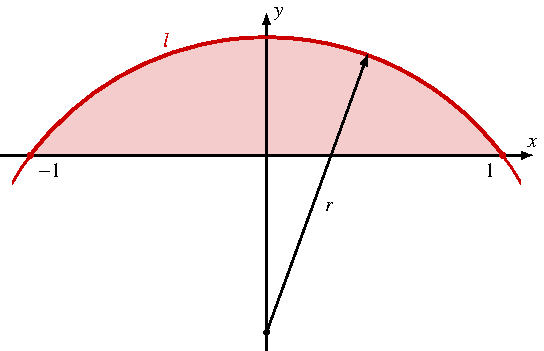
\includegraphics{chapters/050-nebenbedingungen/images/dido.pdf}
\caption{Problem der Dido in der Ebene.
Gesucht wird die Kurve gegebener Länge $l$ zwischen den Punkten $(\pm 1,0)$,
die mit der $x$-Achse den grössten Flächeninhalt einschliesst.
\label{buch:nebenbedingungen:lagrangemult:fig:dido}}
\end{figure}

Gesucht ist eine Funktion $y\colon[-1,1]\to\mathbb{R}$ mit $y(-1)=y(1)=0$
die das Funktional
\[
I(y)
=
\int_{-1}^1 y(x)\,dx
\qquad
\text{mit Lagrange-Funktion}
\qquad
F(x,y,y') = y
\]
extremal macht unter der Nebenbedingung 
\[
J(y)
=
\int_{-1}^1 \sqrt{1+y'(x)^2}\,dx
\qquad
\text{mit Lagrange-Funktion}
\qquad
G(x,y,y') = \sqrt{1+y'^2}.
\]
Die Gradienten sind
\begin{align*}
\grad(F,y)
&=
1
\\
\grad(G,y)
&=
\frac{\partial G}{\partial y}
+
\frac{d}{dx}
\frac{\partial G}{\partial y'}
=
\frac{d}{dx}
\frac{y'(x)}{\sqrt{1+y'(x)^2}}
=
\frac{
y''(x)
}{
(1+y'(x)^2)^{\frac32}
}
\end{align*}
Die Bedingung~\eqref{buch:nebenbedingungen:lagrangemult:notwendig} lautet
jetzt, dass es $\lambda\in\mathbb{R}$ gibt derart, dass
\begin{equation}
1 = \lambda\frac{y''(x)}{(1+y'(x)^2)^{\frac32}}
\qquad\Rightarrow\qquad
\lambda y''(x)= (1+y'(x)^2)^{\frac32}.
\label{buch:nebenbedingungen:lagrangemult:didodgl}
\end{equation}
Wir möchten zeigen, dass die Lösungen der Differentialgleichung
\eqref{buch:nebenbedingungen:lagrangemult:didodgl}
Kreise durch die Punkte $(\pm1, 0)$ sind.
Ein Kreis vom Radius $r$ durch diese beiden Punkte ist der Graph
der Funktion
\[
y(x) = \sqrt{r^2-x^2} - \sqrt{r^2-1}.
\]
Der zweite Term ist konstant und spielt daher in der Differentialgleichung
keine Rolle.
Die ersten beiden Ableitungen von $y(x)$ sind
\begin{align}
y'(x)
&=
-\frac{x}{\!\sqrt{r^2-x^2}}
\quad\Rightarrow\quad
1+y'(x)^2
=
1+\frac{x^2}{r^2-x^2}
=
\frac{r^2}{r^2-x^2}
\notag
\\
y''(x)
&=
-
\frac{
r^2
}{
(r^2-x^2)^{\frac32}
}
=
-\frac{1}{r}
\biggl(
\frac{r^2}{^2-x^2}
\biggr)^{\frac32}
=
-\frac{1}{r}
(1+y'(x)^2)^{\frac32}
\label{buch:nebenbedingungen:lagrangemult:didoloesung}
\end{align}
Die Gleichung \eqref{buch:nebenbedingungen:lagrangemult:didoloesung}
ist die Bedingung \eqref{buch:nebenbedingungen:lagrangemult:didodgl}
mit $\lambda=-r$.
Der Wert, den die Nebenbedingung annimmt, lässt sich jetzt auch
ausrechnen.
Da das Integral $J(y)$ die Länge eines Kreisbogens vom Radius $r$ 
durch die Punkte $(\pm1,0)$ ist, folgt
\[
J(y)
=
2r\arctan\frac{1}{r}
=
-2r\arctan\frac{1}{\lambda}.
\]
Das isoperimetrische Problem wird also lokal von einem Kreisbogen
gelöst.
\end{beispiel}

Aus der lokalen Lösung des isoperimetrischen Problems von Dido
folgt auch, dass die grösste Fläche, die von einer Kurve der Länge
$l$ in der Ebene eingeschlossen werden kann, ein Kreis mit Radius
$r=l/2\pi$ und Flächeninhalt $l^2/4\pi$ ist.
Falls der Bogen zwischen den Punkten $P$ und $Q$ auf einer Kurve, die
den Flächeninhalt maximiert, kein Kreisbogen ist, dann kann man die
Fläche grösser machen, indem man ihn durch durch einen gleichlangen
Kreisbogen ersetzt.
Dieser Widerspruch zeigt, dass die Kurve ein Kreis sein muss.

%
% Laagrange-Multiplikatoren für Variationsprobleme
%
\subsection{Lagrange-Multiplikatoren für Variationsprobleme
\label{buch:nebenbedingungen:lagrangemult:subsection:lagrangemult}}
Die Formulierung der notwendigen Bedingung für ein Extremum eines
Variationsproblems mit einer einzelnen Nebenbedingung kann jetzt
ganz analog wie in Abschnitt~\ref{} für das Minimalproblem für eine
Funktion mehrere Variablen mit Nebenbedingungen verallgemeinert
werden.

\begin{satz}
Seien $F$ und $G_i$ zweimal stetig differenzierbare Funktionen
$[x_1,x_2]\times\mathbb{R}^n\times\mathbb{R}^n\to\mathbb{R}$
und $y\colon[x_1,x_2]\to\mathbb{R}$ eine zweimal stetig
differenzierbare Funktion mit $y(x_1)=y_1$ und $y(x_2)=y_2$, für die
das Funktional
\[
I(y)
=
\int_{x_1}^{x_2} F(x,y(x),y'(x))\,dx
\]
zu einem Extremwert macht unter allen solchen Funktionen, die zusätzlich
die Nebenbedingungen
\[
J_i(y)
=
\int_{x_1}^{x_2}
G_i(x,y(x),y'(x))\,dx,
\quad
i=1,\dots,k,
\]
erfüllen.
Dann gibt es Zahlen $\lambda_i$, $i=1,\dots,k$ derart, dass
\[
\grad(F,y)
=
\lambda_1\grad(G_1,y)+\ldots+\lambda_k\grad(G_k,y)
=
\sum_{i=1}^k \lambda_i \grad(G_i,y)
\]
gilt.
\end{satz}

Ein Extremum des Funktionals $I(y)$ unter den Nebenbedingungen ist
also eine Lösung des Gleichungssystems
\begin{align}
J_i({\color{darkred}y})&=0,\quad i=1,\dots,k\\
\grad(F,{\color{darkred}y})
&=\sum_{i=1}^k {\color{darkred}\lambda_i} \grad(G,{\color{darkred}y})
\end{align}
Dies sind insgesamt $k+1$ Gleichungen für die $k$ reellen Zahlen
${\color{darkred}\lambda_i}\in\mathbb{R}$ und eine unbekannte Funktion
${\color{darkred}y(x)}$.
Die zweite Gleichung ist eine Differentialgleichungen zweiter Ordnung.



